%%%%%%%%%%%%%%%%%%%%%%%%%%%%%%%%%%%%%%%%%
% Stylish Article
% LaTeX Template
% Version 2.1 (1/10/15)
%
% This template has been downloaded from:
% http://www.LaTeXTemplates.com
%
% Original author:
% Mathias Legrand (legrand.mathias@gmail.com) 
% With extensive modifications by:
% Vel (vel@latextemplates.com)
%
% License:
% CC BY-NC-SA 3.0 (http://creativecommons.org/licenses/by-nc-sa/3.0/)
%
%%%%%%%%%%%%%%%%%%%%%%%%%%%%%%%%%%%%%%%%%

%----------------------------------------------------------------------------------------
%	PACKAGES AND OTHER DOCUMENT CONFIGURATIONS
%----------------------------------------------------------------------------------------

\documentclass[fleqn,12pt]{SelfArx} % Document font size and equations flushed left

% \usepackage[english]{babel} % Specify a different language here - english by default

\usepackage[T1]{fontenc}
\usepackage[brazil]{babel}
\usepackage[brazil]{varioref}
\usepackage[utf8]{inputenc}

\usepackage{lipsum} % Required to insert dummy text. To be removed otherwise

%----------------------------------------------------------------------------------------
%	COLUMNS
%----------------------------------------------------------------------------------------

\setlength{\columnsep}{0.55cm} % Distance between the two columns of text
\setlength{\fboxrule}{0.75pt} % Width of the border around the abstract

%----------------------------------------------------------------------------------------
%	COLORS
%----------------------------------------------------------------------------------------

\definecolor{color1}{RGB}{0,0,90} % Color of the article title and sections
\definecolor{color2}{RGB}{0,20,20} % Color of the boxes behind the abstract and headings

%----------------------------------------------------------------------------------------
%	HYPERLINKS
%----------------------------------------------------------------------------------------

\usepackage{hyperref} % Required for hyperlinks

\hypersetup{hidelinks,
            colorlinks,
            breaklinks=true,
            urlcolor=color2,
            citecolor=color1,
            linkcolor=color1,
            bookmarksopen=false,
            pdftitle={Title},
            pdfauthor={Author}
            }

\usepackage[autostyle]{csquotes}
\usepackage[backend=biber]{biblatex}

\addbibresource{sample.bib}

%----------------------------------------------------------------------------------------
%	ARTICLE INFORMATION
%----------------------------------------------------------------------------------------

\JournalInfo{UFRPE, 13/08/2018}
\Archive{Disciplina de computação evolutiva}

\PaperTitle{
União de métodos de processamentos de imagens digitais, que encadeado em
processo de reconhecimento dígitos escritos a mão livre
} % Article title

\Authors{Iury Adones Xavier dos Santos\textsuperscript{1}*,
         Dr. Adenilton Jos\'{e} da Silva\textsuperscript{1},
         Dr. P\'{e}ricles Barbosa Cunha de Miranda\textsuperscript{1},
         Dr. Danilo Ricardo Barbosa de Araújo\textsuperscript{1},
         } % Authors

\affiliation{
\textsuperscript{1}\textit{Programa de Pós-Graduação em Informatica Aplicada (PPGIA), Universidade Federal Rural de Pernambuco (UFRPE), Recife-PE, Brasil}
} % Author affiliation

\affiliation{*\textbf{Autor correspondente}: iuryadones@gmail.com} % Corresponding author

\Keywords{
Algoritmos genéticos --- Processamento encadeado --- Reconhecimento de dígitos 
} % Keywords - if you don't want any simply remove all the text between the curly brackets

\newcommand{\keywordname}{Palavras-chaves} % Defines the keywords heading name

%----------------------------------------------------------------------------------------
%	ABSTRACT
%----------------------------------------------------------------------------------------

\Abstract{
Neste presente trabalho, têm experimentos voltados na área de processamento de
imagens digitais e heurística voltada ao reconhecimento de números escritos, no
entanto, aborda-se alguns passos antes mesmo de chegar-se ao reconhecimento dos
dígitos. Nesses passos que nos revela um fluxo encadeado, são atualmente
produzidos nas literaturas acadêmicas as seções do fluxo de processamento de
imagens, que inicia desda aquisição da imagem bruta, limpeza de ruídos e
binarização dos objetos, pode compor até mesmo com reconhecimento de objetos.
Tais trechos da trajetória do encadeamento, necessita de métodos de otimização,
pois melhoram os resultados, tanto na visualização e classificação. Nós
construirmos experimentos, que testa algumas das possíveis combinações dos
fluxos de encadeamento, estão contidas em um espaço de busca restrito, e nesta
construção abordamos com métodos baseado em algoritmos genéticos, que nos
informa quais as melhores combinações do fluxo encadeado, passadas por avaliação
de minimização do quantitativo de erros na detecção dos dígitos, sem a
necessidade de otimizar cada seção por vez.
}

%----------------------------------------------------------------------------------------

\begin{document}

\flushbottom % Makes all text pages the same height

\maketitle % Print the title and abstract box

\tableofcontents % Print the contents section

\thispagestyle{empty} % Removes page numbering from the first page

%----------------------------------------------------------------------------------------
%	ARTICLE CONTENTS
%----------------------------------------------------------------------------------------
\medskip

\pagebreak

\section*{Introdução} % The \section*{} command stops section numbering

\addcontentsline{toc}{section}{Introdução} % Adds this section to the table of contents

Nos recentes trabalhos têm heurísticas que focam em melhorar as imagens para
depois ter uma segmentação, classificação e reconhecimento de objetos, mas
devido ao progresso nas pesquisas, agora podemos usar uma imagem de entrada e
dizer que espera se na saída como resposta, tal como uma rede neural
supervisionada, no entanto existe uma longa jornada com experimentos e
avaliações, ou seja, até chegarmos nos excelentes resultados. Temos em
\cite{KATKAR2015}, a contribuição na seleção de métodos de pre-processamento
para melhoras nas classificações, e com isso temos entendimento sobre a
identificação de caracteres, dígitos, letras e números em uma imagem, porém se
tivermos uma grande quantidade de imagens identificarmos, tais elementos, isso
será um gasto de tempo e energia mental exorbitante. Foram desenvolvidos
algoritmos que ajudam na redução desses gastos, porém necessita de recursos como
computadores, para tal gasto, por tanto, percebe se que sempre existira um gasto
para tal feito, mas também podemos otimizar tais gastos, no reconhecimento de
dígitos, podemos usar métodos e ou heurísticas dos algoritmos genéticos e ou
evolucionários, logo existem grandes desafios em otimizarmos o nosso gasto
computacional e encontrar a melhor solução para todas as imagens ou grupos de
imagens. 


 % and some mathematics $\cos\pi=-1$ and $\alpha$ in the text\footnote{And some
 % mathematics $\cos\pi=-1$ and $\alpha$ in the text.}.

%------------------------------------------------

\section{Metodologia}

Experimentos baseados no processamento de imagem digital, que iremos abordar
desda aquisição da base, escolhas dos algoritmos de processamento de imagens,
escolha dos algoritmos de binarização até a escolha do método de classificação.

% % Using \begin{figure*} makes the figure take up the entire width of the page
% \begin{figure*}[ht]\centering 
% 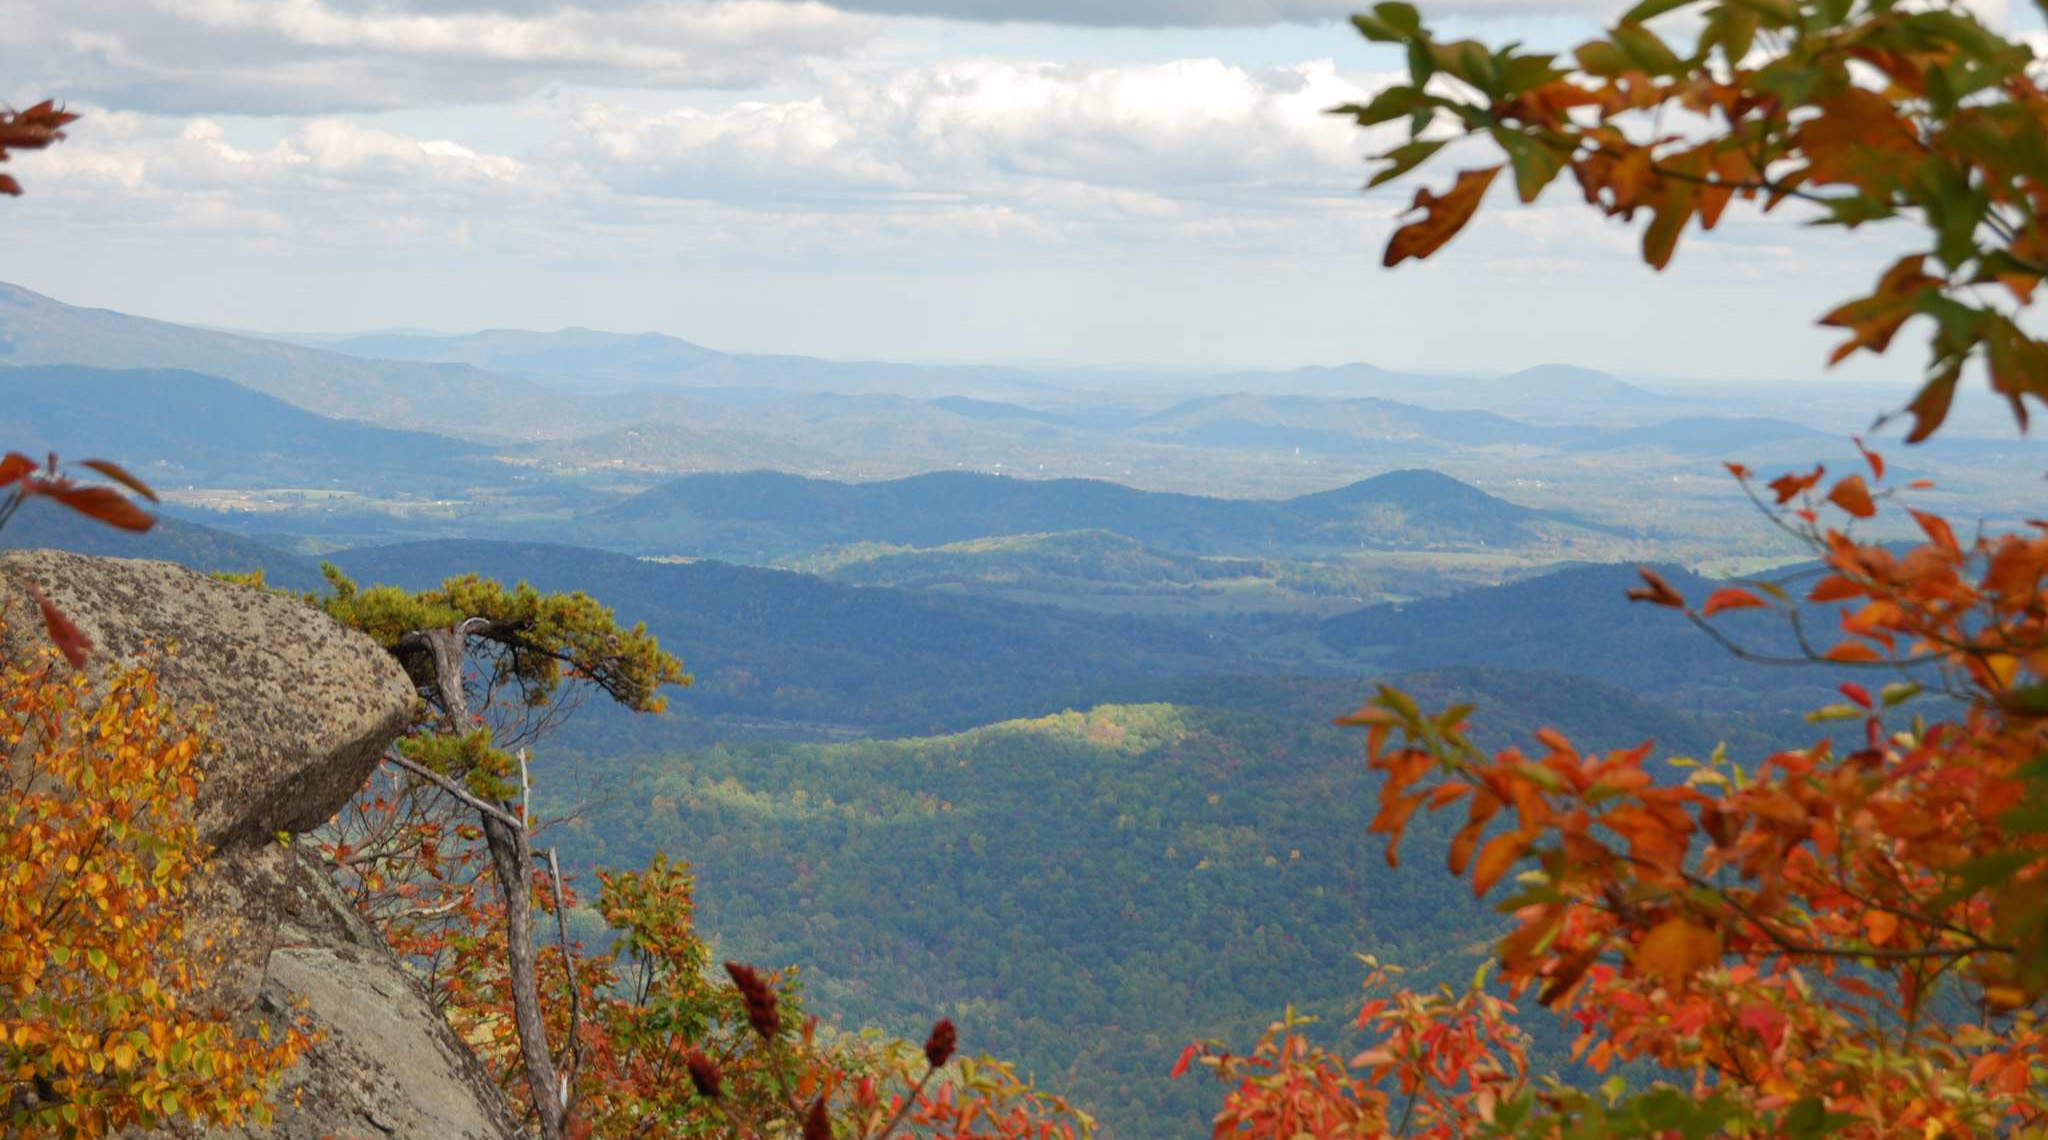
\includegraphics[width=\linewidth]{view}
% \caption{Wide Picture}
% \label{fig:view}
% \end{figure*}

% \begin{equation}
% \cos^3 \theta =\frac{1}{4}\cos\theta+\frac{3}{4}\cos 3\theta
% \label{eq:refname2}
% \end{equation}

% % [noitemsep] removes whitespace between the items for a compact look
% \begin{enumerate}[noitemsep] 
% \item First item in a list
% \item Second item in a list
% \item Third item in a list
% \end{enumerate}

\subsection{Aquisição das imagens de treino}

Usamos a base da MNIST \cite{MNIST2010}, usamos no classificador para treinar, e também as
imagens da MNIST, já são bem conhecida, para pequenos testes e já estão em forma
de binarização, têm umas imagens de escrita a mão livre, com dígitos e de
diferentes tipos de escritas.

\subsection{Elaboração das imagens testes}

Imagens testes foram elaboradas as escritas dos dígitos de forma aleatória,  mas
que fossem próximas as que estão na base da MNIST, visto que nosso objetivo é em
preprocessar as imagens e usar o classificador para os dígitos elaborados e ter
uma classificação satisfatória, mas não é como objetivo principal tal
classificação. Nesta fase de teste de hipótese, de tal, será possível construir
um único fluxo encadeado para o processamento de imagens de diferentes tamanhos
e fontes diferentes, também será possível classificar todos os dígitos contidos
nas imagens só com um único encadeamento? Está é a pergunta que nos move em tal
pesquisa.

\subsection{Escolha do classificador}

 A escolha do classificador, foi usado dois critério que são a velocidade de
treinamento e classificação, e também sua frequência nos periódicos de
classificação de textos, dígitos e caracteres. Escolhemos o máquina de suporte
vetorial, também conhecida como SVM que em inglês é ``suporte vector machine''
\cite{ANIL2015}.

\subsection{Descritor de objeto}

O descritor usado neste trabalho, foi o histograma de gradientes orientados,
conhecido como HOG em inglês é ``Histogram of Oriented Gradients''
\cite{NEWELL2011}. Buscamos usar este descritor, pelo que foi visto sendo usado
em algumas literaturas, mas também nosso objetivo é só classificar objetos nas
imagens testes e de forma mais flexível.

\subsection{Algoritmos de processamento de imagens}

Foram usados um conjuntos de algoritmos, mas que já foram passados por um crivo
de uns periódicos. Tais algoritmos foram de limiarização gaussiana, filtro de
média, filtro gaussiano, algoritmo de Otsu para binarização, também foi usado
binarização invertida, e método adaptativo de binarização por média e com
distribuição gaussiana de acordo com \cite{GUPTA2007}, algoritmo de dilatação e
de erosão, algoritmos de transformação de imagens de três camadas para uma
camada, também conhecida como transformação de tons de cinza.

\subsection{Algoritmo genético}

\{Reference\} Utilizamos nesta pesquisa o algoritmo genético, seguindo um fluxo,
primeiro geração da população de forma aleatória com distribuição uniforme, para
os alelos, temos que alelos são todos os algoritmo de processamento de imagens e
também consideramos seus variantes, no entanto deixamos o primeiro indexe do
alelo como sendo nulo, ou seja, não existe um operador de processamento de
imagem, como fixamos o tamanho da solução em 8 genes e 12 genes, isso faz com
que não necessariamente usaremos os operadores em todos os genes, objetivo é
encontrar a solução ótima, e tal solução é nosso encadeamento.

\subsection{Restrição do algoritmo genético}

\{Reference\} Usamos restrição no gene, que é um dos possíveis operadores de
processamento de imagem, porém existe certos operadores que são usados em
tensores e outros que só se aplicam em matrizes, mas na formação da solução, o
algoritmo que gera não sabe qual é a ordem dos operadores. Para que seja
executados todos corretamente, no entanto, abordamos dois tipos de restrições,
uma que se tiver no gene um operador que não consiga ser executado, então passe
para o prosseguimos e a informação daquela solução será passada para a próximas
geração, já a outra como somos especialista, colocamos as imagens já no formato
de matrizes para não tenha uma passagem forçada, pois sabemos que todos outros
operadores, conseguem processar em matrizes, mas só alguns que conseguem em
tensores.


%------------------------------------------------

\section{Resultados e Análise}

Conseguimos alguns indicadores que poderemos contribuir com a comunidade
acadêmica, tais indicadores são no pre processamento das imagens antes mesmo de
classificação dos objetos contidas, ou seja, uma preparação da imagem ou um
conjunto de imagens para único tipo de encadeamento. 

\pagebreak

\subsection{Experimento - 1}

\begin{figure}[ht]\centering
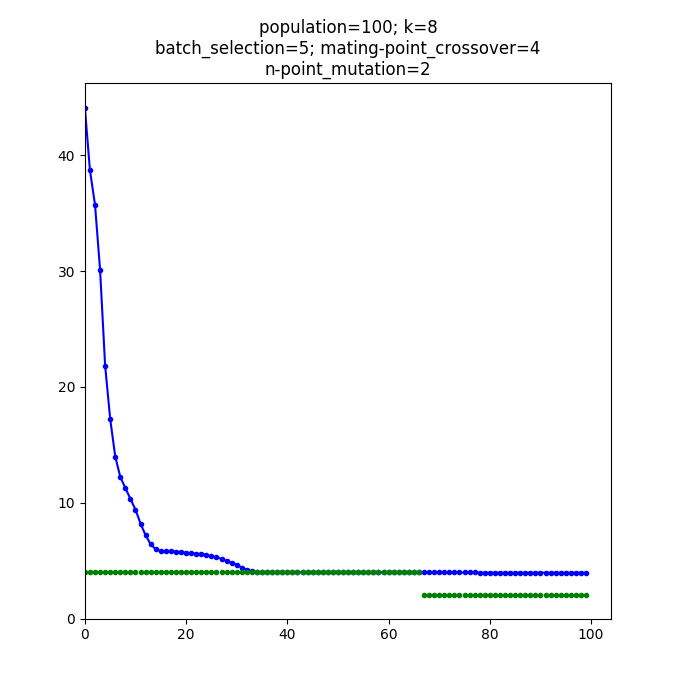
\includegraphics[width=\linewidth]{./experiments/media_and_steps_8_op_8}
\caption{Solução com 8 passos de encadeados de processamento e tendo cada passo
8 operadores possíveis de escolha, sem restrição da solução.}
\label{fig:media_and_steps_8_op_8}
\end{figure}

\medskip
\medskip
\medskip
\medskip
\medskip
\medskip
\medskip
\medskip
\medskip
\medskip
\medskip
\medskip
\medskip
\medskip
\medskip
\medskip
\medskip
\medskip
\medskip
\medskip

\pagebreak

\subsection{Experimento - 2}

\begin{figure}[ht]\centering
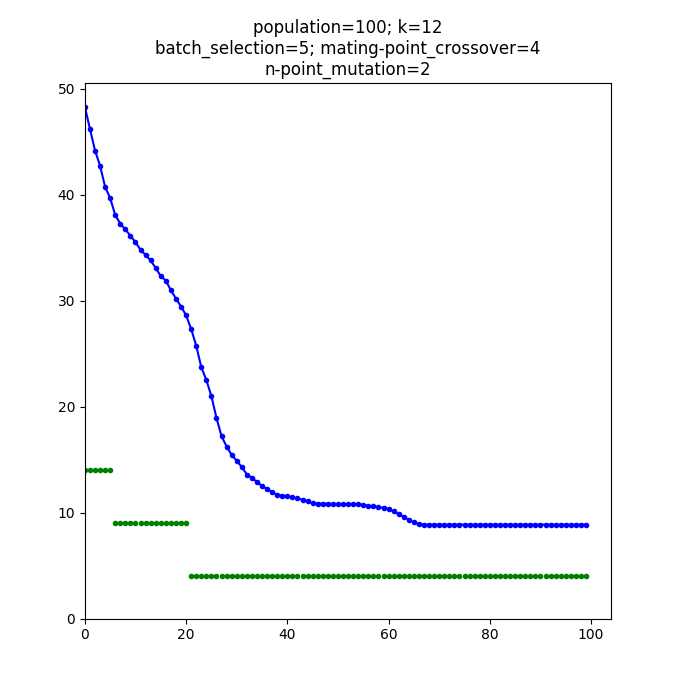
\includegraphics[width=\linewidth]{./experiments/media_steps_12_op_20}
\caption{Solução com 12 passos de encadeados de processamento e tendo cada passo
20 operadores possíveis de escolha, com restrição de passar para o próximo
operador do encadeamento.}
\label{fig:media_steps_12_op_20}
\end{figure}

\medskip
\medskip
\medskip
\medskip
\medskip
\medskip
\medskip
\medskip
\medskip
\medskip
\medskip
\medskip
\medskip
\medskip
\medskip
\medskip
\medskip
\medskip
\medskip
\medskip
\medskip
\medskip
\medskip
\medskip

\pagebreak

\subsection{Experimento - 3}

\begin{figure}[ht]\centering
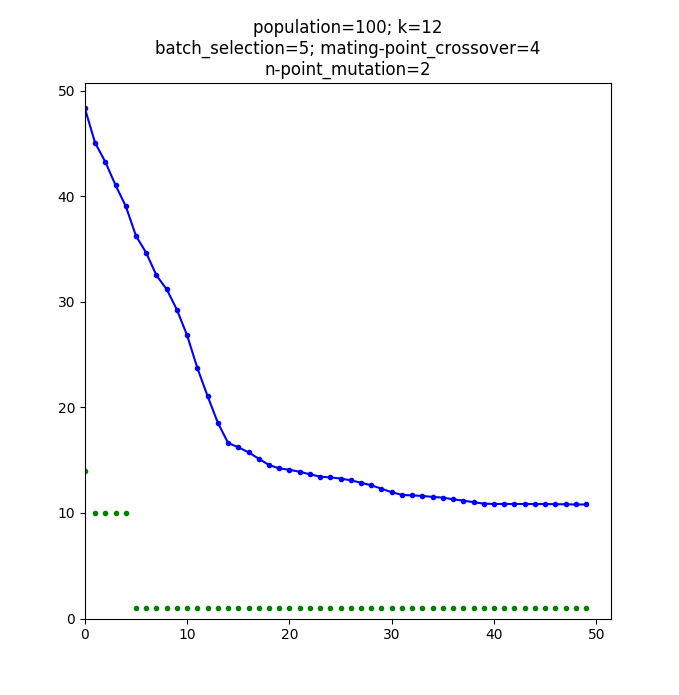
\includegraphics[width=\linewidth]{./experiments/media_and_steps_12_op_20_step_50}
\caption{Solução com 12 passos de encadeados de processamento e tendo cada passo
20 operadores possíveis de escolha, com restrição do especialista que transforma
inicialmente a imagem tensorial para matriz na escala de cinza.}
\label{fig:media_and_steps_12_op_20_step_50}
\end{figure}


Observamos que podemos usar uma heurística para pre-processamento de imagens de
forma a servir para diversas imagens da mesma classe de problema, de acordo com
os resultados apresentados na figura \ref{fig:media_and_steps_12_op_20_step_50},
que chega apenas errar um digito na imagem, sabendo que o conjunto é de 40
dígitos.



%------------------------------------------------


\phantomsection
\section*{Agradecimentos}

\addcontentsline{toc}{section}{Agradecimentos}

Agradeço a todos que contribuíram com o projeto.

%----------------------------------------------------------------------------------------
%	REFERENCE LIST
%----------------------------------------------------------------------------------------
\phantomsection
\addcontentsline{toc}{section}{Referência}

\printbibliography 
%----------------------------------------------------------------------------------------

\end{document}